
\section{Algorithms}


\subsection{Using full models}
I have implemented an algorithm that uses higher order models to approximate the constraints.

In this algorithm, we add additional degrees of freedom to the constraints to cut off points that have been evaluated and are infeasible.
The models are forced to be a given negative value at these points.

One question for this method is how many constraints to model.


I implemented Kriging, as this can use as many points as are available.
However, this requires using some artificial value of the constraints at infeasible points.

\subsection{Using linear models}

Another method is to add additional linear constraints each time a new point is evaluated and infeasible.

Each new linear constraint cuts off an infeasible point and stays atleast a fraction of the trust region away from that infeasible point.


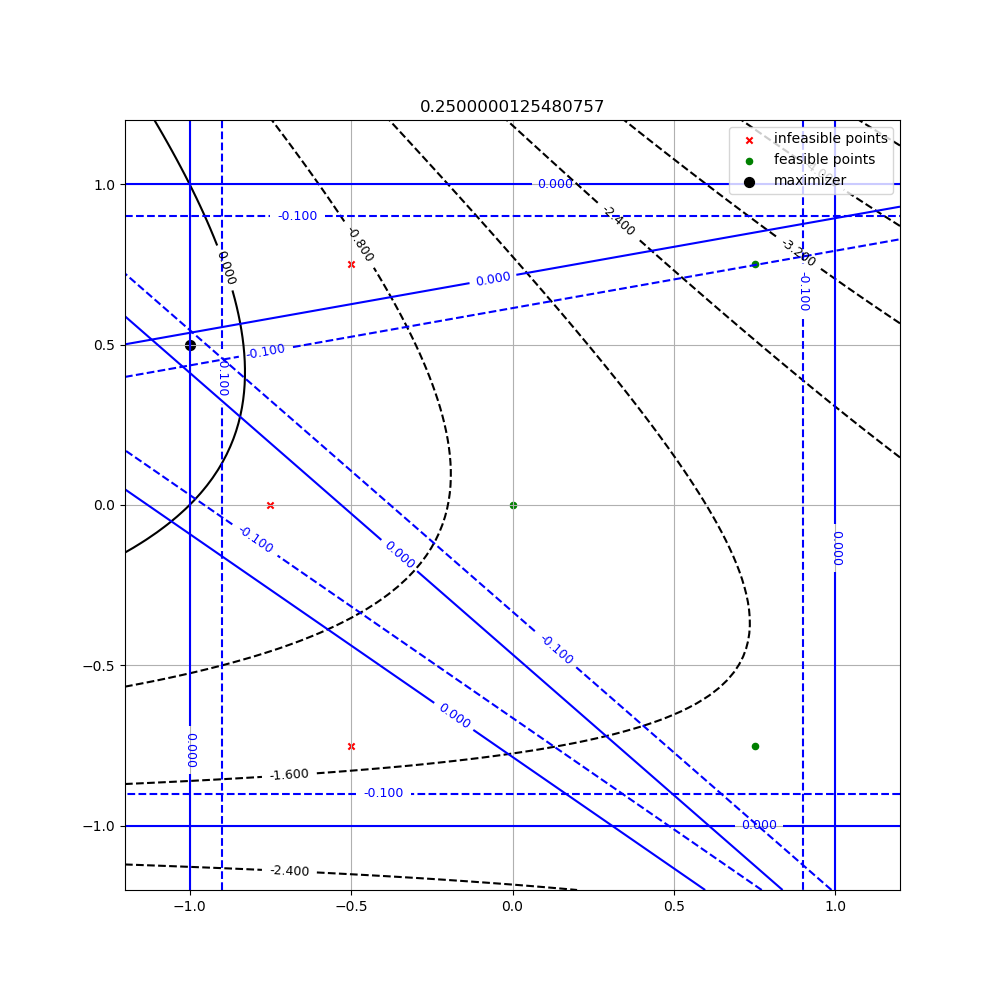
\includegraphics[width=300px]{images/pyomo_cut_solution.png}

\subsubsection{formulation}

The optimization program for finding this constraint is given by:

A set of $u^i, 1 \le i \le n_{I}$ infeasible points.
A set of $v^i, 1 \le i \le n_{F}$ feasible points.

The current Lagrange polynomial $\frac 1 2 x^T Q x + b^Tx$.
Require all infeasible point to be a distance at least $d$ from the feasible region.


Find a set of planes $(n^i, b^i), 1 \le i \le n_{P}$.

Require $n_P \ge n_I$.


What we want big:
\begin{align}
\max_{x} & \frac 1 2 x^T Q x + b^Tx &\\
 & {n^i}^T x \le b^i & \forall 1 \le i \le n_{P} \\
 & {n^i}^T v_j \le b^i & \forall 1 \le i \le n_{P}, 1\le j\le  n_{F} \\
 & {n^i}^T u_i \ge b^i + d & \forall 1 \le i \le n_{I} \\
 & \| n^i \| = 1 & \forall 1 \le i \le n_{I} \\
 & 0 \le x_i \le 1 & \forall 1 \le i \le n \\
\end{align}


A set of $v_i, 1 \le i \le n_{I}$ feasible points.




\subsection{Using a sacred region}


\begin{itemize}
    \item Define a suitable ellipsoid to be an ellipsoid that satisfies the following conditions: \begin{itemize}
        \item It can be scaled by a factor of 2 to include the current iterate.
        \item It touches a boundary of the current trust region
        \item It has bounded condition number (which happens because of one of the following)
        \item One of the following two  \begin{itemize}
            \item \begin{itemize}
                \item It either touches a constraint
                \item The center lies on $\hat u$ of the previous iteration
                \item It has two singular values
            \end{itemize}
        \end{itemize}
        \item It has condition number 1
    \end{itemize}
\end{itemize}



\begin{algorithm}[H]
    \caption{Construct next trust region}
    \label{constrained_dfo}
    \begin{itemize}
        \item[\textbf{Step 0}] \textbf{(Initialization)} \\
            Given the current \begin{itemize}
                \item[] trust region $\dk$
                \item[] ellipse $E_k$
                \item[] sample points
                \item[] model functions
            \end{itemize}
        
        \item[\textbf{Step 1}] \textbf{(Check stopping criteria)} \\
            Evaluate the next iterate \begin{itemize}
                \item[] If $\rho_k < \gammasm$ then $\iteratekpone=\iteratek$ (reject) and $\Delta_{k+1} = \omegadec\Delta_{k}$
                \item[] Otherwise, get temp cone
                \item[] if the temp cone hits a model of the constraint, decrease the next trust region get temp ellipsoid    
                \item[] reshape ellipse
            \end{itemize}
        
        \item[\textbf{Step 2}] \textbf{(Construct sample set in temp ellipsoid)} \\
            If a point in the temp ellipse is infeasible, then reject and decrease trust region
            % \item[] This can also be $\trialk = \min_{s \in \outertrk \cap \feasiblek} \modelk(\iteratek + \trialk)$ depending on the choice made in \cref{which_trust_region}.
            
        \item[\textbf{Step 3}] \textbf{(Move to temp ellipse)} \\
            Evaluate $f(\iteratek + \trialk)$ and evaluate $\rho_k$ as in \cref{rho} \begin{itemize}
                \item[] $\iteratekpone=\iteratek+\trialk$ (accept), $\Delta_{k+1} = \omegadec\Delta_{k}$
                \item[] $\Delta_{k+1} = $ temp radius
                % and either increase the radius or decrease if $\nabla \modelk(\iteratek)$ is small
            \end{itemize}
            
            
        $k \gets k+1$ and go to Step 1.
    \end{itemize}
\end{algorithm}






Another approach is to ensure that we will always have a large enough feasible region within the current trust region.
This is the approach that we currently have a convergence proof for.


\begin{align*}
\max_{t \in \mathbb R, c \in \mathbb R^n} t \\
\| \xk - c\| \le t \\
\| {x_{inf}}_i - c \| \ge t \quad \forall i
\end{align*}



Assume that the constraints are always linearly independent.
\begin{align*}
\|\nabla c(\xk)\| \ge \reg \forall k\\
\|\nabla m_{c_{i}}(\xk)\| \ge \reg \forall k
\end{align*}


Define
\begin{align*}
\mathcal A(c;x) = \{i =  1,\ldots, n| c_i(x) = 0\}  \quad \forall x \in \feasible \\
\feasdir(c;x) = -\nabla c_{\mathcal A(c;x)}(x)^T(\nabla c_{\mathcal A(c;x)}(x)\nabla c_{\mathcal A(c;x)}(x)^T)^{-1} e \quad \forall x \in \feasible,\mathcal A(c;x) \ne \emptyset \\
\hfeasdir(c;x) = \frac {\feasdir(c;x)} {\| \feasdir (c;x)\|}\\
\nabla \hat c_i(x) = \frac {\nabla c_i(x)}{\|\nabla c_i(x)\|} \forall i\\
\alpha_1(c;x) =
\begin{cases}
-\max_{i \in \mathcal A(c;x)} \nabla \hat c_i(x) \hfeasdir(c;x) & \text{if} \quad \mathcal A(c;x) \ne \emptyset \\
\infty & \text{if} \quad \mathcal A(c;x) = \emptyset
\end{cases} \\
\alpha_2(c;x) =
\begin{cases}
\max_{t > 0} c(x + t\hfeasdir(c;x)) \le 0 & \text{if} \quad \mathcal A(c;x) \ne \emptyset \\
\infty & \text{if} \quad \mathcal A(c;x) = \emptyset
\end{cases} \\
C(c, u, \alpha) = \{x \in \mathbb R^n | \quad x = c + t u + s, s^T u = 0, t > 0, \|s\| \le \alpha t\} \\
\end{align*}


\begin{theorem}
There exists an $\epsilon > 0$ such that $\alpha_1(x) > \epsilon$ for all $x \in \feasible$.
\end{theorem}

\begin{proof}
\end{proof}


During iteration $k$, define
\begin{align*}
u^{(k)} = \hfeasdir(\modelconstraint, \iteratekpone) \\
\alpha_1^k = \alpha_1(\modelconstraint, \iteratekpone) \\
\alpha_2^k = \alpha_2(\modelconstraint, \iteratekpone) \\
\mathcal A_k = \mathcal A(\modelconstraint, \iteratekpone) \\
C_k = C\left(\iteratekpone + \dbuf\dk u^{(k)}, u^{(k)}, \abuf\alpha_1^k\right). \\
\end{align*}

\begin{theorem}
Let $\dbuf \in (0, 1), \abuf \in (0, 1)$.
If
\begin{align*}
\dk \le \min\left\{
\sqrt{\frac{(1 - \abuf) \alpha_1^k}{\epsilon_g(1 + \abuf\alpha_1^k)}},
\sqrt{\alpha_1^k \left(\epsilon_g + \frac{\epsilon_f}{\dbuf}\right)^{-1}}
\right\},
\end{align*}
then $B_{\infty}(\iteratekpone, \dk)\cap C_k \subseteq \feasible.$
\end{theorem}

\begin{proof}


Let $y \in B_{\infty}(\iteratekpone, \dk)\cap C_k$, so that
\begin{align*}
y = \iteratekpone + \dbuf\dk u^{(k)} + tu^{(k)} + s \\
\|s\| \le t \abuf\alpha_1^k \\
s^Tu^{(k)} = 0.
\end{align*}
Let $i \in \mathcal A_k$ be arbitrary.
We know that there exist $\mu,\nu^i\in\mathbb R^n$ with $|\mu_j| \le 1\forall j, \|\nu^i\|\le 1$ such that
\begin{align*}
c_i(\iteratekpone) = m_{c_i}(\iteratekpone) + \epsilon_f \dk^3 \mu^i \\
\nabla c_i(y) = \nabla m_{c_i}(y) + \epsilon_g \dk^2 \nu^i
\end{align*}


By the assumptions,
\begin{align*}
\dk \le \sqrt{\frac{(1 - \abuf) \alpha_1^k}{\epsilon_g(1 + \abuf\alpha_1^k)}}\\
\dk^2  \le \frac{(1 - \abuf) \alpha_1^k}{\epsilon_g(1 + \abuf\alpha_1^k)}\\
\epsilon_g \dk^2 (1 + \abuf\alpha_1^k) \le (1 - \abuf) \alpha_1^k\\
-t(1 - \abuf) \alpha_1^k + \epsilon_g t\dk^2 (1 + \abuf\alpha_1^k) \le 0.
\end{align*}

From there,
\begin{align*}
\nabla \hat c_{i}^T(\iteratekpone)(tu^{(k)} + s) = 
\nabla \hat {m_c}_{i}^T(tu^{(k)} + s) + \epsilon_g \dk^2 {\nu^i}^T(tu^{(k)} + s) \\
=t\nabla \hat {m_c}_{i}^Tu^{(k)} + \nabla \hat {m_c}_{i}^Ts + \epsilon_g \dk^2 (t + \|s\|) \\
\le -t \alpha_1^k + \|s\| + \epsilon_g \dk^2 (t + t \abuf\alpha_1^k) \\
\le -t \alpha_1^k + t \abuf \alpha_1^k  + \epsilon_g t\dk^2 (1 + \abuf\alpha_1^k) \\
\le -t(1 - \abuf) \alpha_1^k  + \epsilon_g t\dk^2 (1 + \abuf\alpha_1^k) \le 0.
\end{align*}


% \begin{align*}
% \nabla m_{c_i}^T(\iteratekpone)u^{(k)} \le \max_i \nabla m_{c_i}^T(\iteratekpone)u^{(k)} \\
% -\nabla m_{c_i}^T(\iteratekpone)u^{(k)} \ge -\max_i \nabla m_{c_i}^T(\iteratekpone)u^{(k)} \\
% -\nabla m_{c_i}^T(\iteratekpone)u^{(k)} \ge \alpha_1^k \\
% \alpha_1^k \le -\nabla m_{c_i}^T(\iteratekpone)u^{(k)}\label{aaaaaaaa_1}. \\
% \end{align*}

Also by the assumptions,
\begin{align*}
\dk \le \sqrt{\alpha_1^k \left(\epsilon_g + \frac{\epsilon_f}{\dbuf}\right)^{-1}} \\
\dk^2 \le \alpha_1^k \left(\epsilon_g + \frac{\epsilon_f}{\dbuf}\right)^{-1} \\
\dk^2(\epsilon_g + \frac{\epsilon_f}{\dbuf}) \le \alpha_1^k \le -\nabla m_{c_i}^T(\iteratekpone)u^{(k)}\\
\nabla m_{c_i}^T(\iteratekpone)u^{(k)} + \dk^2(\epsilon_g + \frac{\epsilon_f}{\dbuf}) \le 0\\
\dbuf\nabla m_{c_i}^T(\iteratekpone)u^{(k)} + \dk^2(\epsilon_g \dbuf + \epsilon_f) \le 0.
\end{align*}

From there,


\begin{align*}
\epsilon_f \dk^3 \mu_i + \nabla {c}^T_{i}(\iteratekpone)\dbuf\dk u^{(k)} = 
\epsilon_f \dk^3 \mu_i + (\nabla m_{c_i}(\iteratekpone) + \epsilon_g \dk^2 \nu^i)^T\dbuf\dk u^{(k)} \\
= \epsilon_f \dk^3 \mu_i + \dbuf\dk\nabla m_{c_i}^T(\iteratekpone)u^{(k)}  + \epsilon_g \dk^3 \dbuf {\nu^i}^Tu^{(k)} \\
\le \dk\left(\dbuf\nabla m_{c_i}^T(\iteratekpone)u^{(k)} + \dk^2(\epsilon_g \dbuf + \epsilon_f)\right) \le 0.
\end{align*}


Finally,
\begin{align*}
c_{\mathcal A_k}(y) = c_{\mathcal A_k}(\iteratekpone) + \nabla {c}^T_{\mathcal A_k}(\iteratekpone)(y - \iteratekpone) + \xi \\
= m_{c_{\mathcal A_k}}(\iteratekpone) + \epsilon_f \dk^3 \mu^{\mathcal A_k} + \nabla {c}^T_{\mathcal A_k}(\iteratekpone)(y - \iteratekpone) + \xi \\
= \epsilon_f \dk^3 \mu^{\mathcal A_k} + \nabla {c}^T_{\mathcal A_k}(\iteratekpone)(y - \iteratekpone) + \xi \\
= \epsilon_f \dk^3 \mu^{\mathcal A_k} + \nabla {c}^T_{\mathcal A_k}(\iteratekpone)\dbuf\dk u^{(k)} + 
\|\nabla {c}^T_{\mathcal A_k}(\iteratekpone)\| \nabla \hat{c}^T_{\mathcal A_k}(\iteratekpone)(tu^{(k)} + s) + \xi  \\
\le \xi.
\end{align*}
% \nabla \hat {c}_{\mathcal A_k}(\iteratekpone)^T(\dbuf\dk u^{(k)} + tu^{(k)} + s) = 





% 
% \begin{align*}
% \nabla \hat c_{\mathcal A_k}^T(y - \iteratekpone) = 
% \nabla \hat {m_c}_{\mathcal A_k}^T(\dbuf\dk u^{(k)} + tu^{(k)} + s) + \epsilon_f \dk^3 \nu^T(\dbuf\dk u^{(k)} + tu^{(k)} + s) \\
% \le \nabla \hat {m_c}_{\mathcal A_k}^T(\dbuf\dk u^{(k)} + tu^{(k)} + s) + \epsilon_f \dk^3 \nu^T(\dbuf\dk u^{(k)} + tu^{(k)} + s) \\
% \end{align*}

% \le t \nabla \hat {m_c}_{\mathcal A(\modelconstraint, \xk)}^T\hfeasdir(\xk) + \nabla \hat {m_c}_{\mathcal A(\modelconstraint, \xk)}^T s + \epsilon_f \dk^3(t + \|s\|) \\
% \le \|s\| - t \alpha_1(\modelconstraint, \xk)+ 2\epsilon_f \dk^4\\
% \le t(1-\dbuf)\alpha_1(\modelconstraint, \xk) - t \alpha_1(\xk)+ 2\epsilon_f \dk^4\\
% \le -t\dbuf\alpha_1(\modelconstraint, \xk) + 2\epsilon_f \dk^4 \\

\end{proof}



\begin{theorem}
Let $m$ be the number of constraints that intersect the trust region.
For sufficiently small $\dk$, the number of subsets $S$ of $\{1, 2, \ldots, m\}$
whose constraints have linearizations that intersect is either 1 or 0.
\end{theorem}

\begin{proof}
\end{proof}



\begin{align*}
m_{c_i}(y) = m_{c_i}(\xk) + \nabla m_{c_i}(\xk)^T(y - \xk) \\
m_{c_i}(\xk - t \nabla m_{c_i}(\xk)) = m_{c_i}(\xk) + \nabla m_{c_i}(\xk)^T(\xk - t \nabla m_{c_i}(\xk) - \xk) = 0 \\
m_{c_i}(\xk) = t\|\nabla m_{c_i}(\xk)\|^2 \\
t = \frac {m_{c_i}(\xk)}{\|\nabla m_{c_i}(\xk)\|^2} \\
m_{c_i}\left(\xk - \frac {m_{c_i}(\xk)}{\|\nabla m_{c_i}(\xk)\|^2} \nabla m_{c_i}(\xk)\right) = 0
\end{align*}

\begin{theorem}
Let $\alpha \in (0, 1)$, $\beta \in (0, 1)$ be given.
Define the cone $C_i$ as:
\begin{align*}
C_i = \left\{x | x = \xk - (1 - \alpha\dk^p)\frac {m_{c_i}(\xk)}{\|\nabla m_{c_i}(\xk)\|^2} \nabla m_{c_i}(\xk) - t\frac{\nabla m_{c_i}(\xk)}{\|\nabla m_{c_i}(\xk)\|} + s,s^T\nabla m_{c_i}(\xk)=0, \|s\| \le (1 - \beta\dk^{-2})t \right\}
\end{align*}
There exists an $\epsilon$, such that if $\dk < \epsilon$ and $|m_{c_i}(\xk)| \le \dk\|\nabla m_{c_i}(\xk)\|$,
then $y \in C_i \cap B_{\infty}(\xk, \dk) \Longrightarrow c_i(y) \le 0$.
\end{theorem}

\begin{proof}
Let $y$ be as defined, and $M \ge \sup_{x \in B_{\infty}(\xk, \dk)} \frac 1 2 \nabla^2 c_i(x)$.
There exists a $\nu \in \mathbb R^n$, $\|\nu\|=1$ such that 
\begin{align*}
\nabla c_i(\xk) = \nabla m_{c_i}(\xk) + \epsilon_{g}\dk^2\nu.
\end{align*}


\begin{align*}
c_i(y) = c_i(\xk) + \nabla c_i(\xk)^T(y - \xk) + \frac 1 2 (y - \xk)^T\nabla^2c_i(\xi) (y - \xk) \\
c_i(y) - \frac 1 2 (y - \xk)^T\nabla^2c_i(\xi) (y - \xk) = c_i(\xk) + \nabla c_i(\xk)^T(y - \xk) \\
= c_i(\xk) + \nabla c_i(\xk)^T(y - \xk + \frac{c_i(\xk)}{\|\nabla c_i(\xk)\|^2}\nabla c_i(\xk) + \xk - \frac{c_i(\xk)}{\|\nabla c_i(\xk)\|^2}\nabla c_i(\xk)- \xk) \\
= \nabla c_i(\xk)^T(y - \xk + \frac{c_i(\xk)}{\|\nabla c_i(\xk)\|^2}\nabla c_i(\xk) - \xk)\\
= \nabla c_i(\xk)^T(\xk - (1 - \alpha\dk^{\frac 1 2})\frac {m_{c_i}(\xk)}{\|\nabla m_{c_i}(\xk)\|^2} \nabla m_{c_i}(\xk) - t\frac{\nabla m_{c_i}(\xk)}{\|\nabla m_{c_i}(\xk)\|} + s - \xk + \frac{c_i(\xk)}{\|\nabla c_i(\xk)\|^2}\nabla c_i(\xk) - \xk) \\
= \nabla c_i(\xk)^T \left(\xk -\frac {m_{c_i}(\xk)}{\|\nabla m_{c_i}(\xk)\|^2} \nabla m_{c_i}(\xk)- \xk + \frac{c_i(\xk)}{\|\nabla c_i(\xk)\|^2}\nabla c_i(\xk) \right) \\
+ \nabla c_i(\xk)^T(\alpha\dk^{\frac 1 2}\frac {m_{c_i}(\xk)}{\|\nabla m_{c_i}(\xk)\|^2} \nabla m_{c_i}(\xk) - t\frac{\nabla m_{c_i}(\xk)}{\|\nabla m_{c_i}(\xk)\|} + s  - \xk)
\end{align*}



% \le m_{c_i}(\xk) + \nabla c_i(\xk)^T(y - \xk) + M \|y - \xk\|^2 \\
% \le m_{c_i}(\xk) + \nabla c_i(\xk)^T((1 - \alpha\dk)\frac {m_{c_i}(\xk)}{\|\nabla m_{c_i}(\xk)\|^2} \nabla m_{c_i}(\xk) + t\frac{\nabla m_{c_i}(\xk)}{\|\nabla m_{c_i}(\xk)\|} + s) + M \|y - \xk\|^2

\begin{align*}
\dk \le \sqrt{\frac {1 + \delta} {2\epsilon_{g}}} \\
2\dk^2 - \beta \le \frac{1 + \delta}{\epsilon_{g}} \\
\dk^2(2 - \beta\dk^{-2}) \le \frac{1 + \delta}{\epsilon_{g}} \\
\epsilon_{g}\dk^2(t +  (1 - \beta\dk^{-2})t) \le t + \delta t \\
\epsilon_{g}\dk^2(t + \|s\|) \le t + \delta t\\
- \epsilon_{g}\dk^2\nu^T(t\frac{\nabla m_{c_i}(\xk)}{\|\nabla m_{c_i}(\xk)\|} + s) \le t + \delta t \\
-t - \epsilon_{g}\dk^2\nu^T(t\frac{\nabla m_{c_i}(\xk)}{\|\nabla m_{c_i}(\xk)\|} + s) \le \delta t \\
(\nabla m_{c_i}(\xk) + \epsilon_{g}\dk^2\nu)^T(- t\frac{\nabla m_{c_i}(\xk)}{\|\nabla m_{c_i}(\xk)\|} + s) \le \delta t \\
\nabla c_i(\xk)^T(- t\frac{\nabla m_{c_i}(\xk)}{\|\nabla m_{c_i}(\xk)\|} + s) \le \delta t \\
\end{align*}



\begin{align*}
\dk^{\frac 1 2} \le \frac{\alpha+\delta}{\sqrt{2}\epsilon_{g}}\|\nabla c_i(\xk)\|^2\\
\dk^{2} \le \dk^{\frac 1 2}\frac{\alpha+\delta}{\sqrt{2}\epsilon_{g}}\dk\|\nabla c_i(\xk)\|^2 \\
\dk^{2} \le\dk^{\frac 1 2} \frac{(\alpha + \delta)}{\sqrt{2}\epsilon_{g}}\frac{\|\nabla m_{c_i}(\xk)\|}{|m_{c_i}(\xk)|}\|\nabla c_i(\xk)\|^2\\
2\epsilon_{g}^2\dk^4
\le (\dk^{\frac 1 2}(\alpha + \delta))^2\frac{\|\nabla m_{c_i}(\xk)\|^2}{|m_{c_i}(\xk)|^2}\|\nabla c_i(\xk)\|^4\\
\epsilon_{g}^2\dk^4
+\left\|\|\nabla m_{c_i}(\xk)\|^2 - \|\nabla m_{c_i}(\xk)\|^2 + \epsilon_{g}\dk^2\|\nu \|^2 \right\|^2
\le (\dk^{\frac 1 2}(\alpha + \delta))^2\frac{\|\nabla m_{c_i}(\xk)\|^2}{|m_{c_i}(\xk)|^2}\|\nabla c_i(\xk)\|^4\\
\|\nabla m_{c_i}(\xk)\|^2\left\|\nabla c_i(\xk) - \nabla m_{c_i}(\xk)\right\|^2
+\|\nabla m_{c_i}(\xk)\|^2\left|\|\nabla m_{c_i}(\xk)\|^2 - \|\nabla c_i(\xk)\|^2
\right|^2\\
\le \frac{(\dk^{\frac 1 2}(\alpha + \delta))^2}{|m_{c_i}(\xk)|^2}\|\nabla m_{c_i}(\xk)\|^4\|\nabla c_i(\xk)\|^4\\
\left\|\nabla c_i(\xk)\|\nabla m_{c_i}(\xk)\|^2 - \nabla m_{c_i}(\xk)\|\nabla m_{c_i}(\xk)\|^2\right\|^2
+\left\|\nabla m_{c_i}(\xk)\|\nabla m_{c_i}(\xk)\|^2 - \nabla m_{c_i}(\xk)\|\nabla c_i(\xk)\|^2
\right\|^2\\
\le \frac{\dk^{\frac 1 2}(\alpha + \delta)}{|m_{c_i}(\xk)|}\|\nabla m_{c_i}(\xk)\|^2\|\nabla c_i(\xk)\|^2\\
\left\|\nabla c_i(\xk)\|\nabla m_{c_i}(\xk)\|^2 - \nabla m_{c_i}(\xk)\|\nabla m_{c_i}(\xk)\|^2
+\nabla m_{c_i}(\xk)\|\nabla m_{c_i}(\xk)\|^2 - \nabla m_{c_i}(\xk)\|\nabla c_i(\xk)\|^2
\right\|\\
\le  \frac{(\dk^{\frac 1 2}(\alpha + \delta))^2}{|m_{c_i}(\xk)|^2}\|\nabla m_{c_i}(\xk)\|^4\|\nabla c_i(\xk)\|^4\\
\left\|\nabla c_i(\xk)\|\nabla m_{c_i}(\xk)\|^2 -
\nabla m_{c_i}(\xk)\|\nabla c_i(\xk)\|^2
\right\| \le \frac{\dk^{\frac 1 2}(\alpha + \delta)}{|m_{c_i}(\xk)|}\|\nabla m_{c_i}(\xk)\|^2\|\nabla c_i(\xk)\|^2\\
\left\|\nabla c_i(\xk)\|\nabla m_{c_i}(\xk)\|^2 -
\nabla m_{c_i}(\xk)\|\nabla c_i(\xk)\|^2
\right\| \le \frac{\dk^{\frac 1 2}(\alpha + \delta)}{|m_{c_i}(\xk)|}\|\nabla m_{c_i}(\xk)\|^2\|\nabla c_i(\xk)\|^2\\
\left\|\frac{\nabla c_i(\xk)}{\|\nabla c_i(\xk)\|^2} -
\frac{\nabla m_{c_i}(\xk)}{\|\nabla m_{c_i}(\xk)\|^2}
\right\| \le \frac{\dk^{\frac 1 2}(\alpha + \delta)}{|m_{c_i}(\xk)|}\\
\|
\xk - \frac{c_i(\xk)}{\|\nabla c_i(\xk)\|^2}\nabla c_i(\xk) -
\xk + \frac{m_{c_i}(\xk)}{\|\nabla m_{c_i}(\xk)\|^2}\nabla m_{c_i}(\xk)
\| \le \dk^{\frac 1 2}(\alpha + \delta)\\
\end{align*}


\begin{theorem}
Let $c_i$ be a constraint that intersects $B_{\infty}(\xk, \dk)$.
\end{theorem}

\begin{proof}
\end{proof}


% \begin{align*}
% \dk^{2-p} - \epsilon_g\dk^2\frac{\alpha}{\sqrt{2}\epsilon_{g}}
% \frac{\|\nabla m_{c_i}(\xk)\|}{|m_{c_i}(\xk)|} \le \frac{\alpha}{\sqrt{2}\epsilon_{g}}
% \frac{\|\nabla m_{c_i}(\xk)\|}{|m_{c_i}(\xk)|}\|\nabla m_{c_i}(\xk)\|^2\\
% \left\|\frac{\nabla c_i(\xk) \|\nabla m_{c_i}(\xk)\|^2 - \nabla m_{c_i}(\xk)\|\nabla c_i(\xk)\|^2}{\|\nabla c_i(\xk)\|^2\|\nabla m_{c_i}(\xk)\|^2}
% \right\| \le \frac{\alpha \dk}{|m_{c_i}(\xk)|}\\
% \left\|\nabla c_i(\xk) \|\nabla m_{c_i}(\xk)\|^2 - \nabla m_{c_i}(\xk)\|\nabla c_i(\xk)\|^2
% \right\| \le \|\nabla c_i(\xk)\|^2\|\nabla m_{c_i}(\xk)\|^2 \frac{\alpha \dk}{|m_{c_i}(\xk)|}\\
% \left\|( \nabla m_{c_i}(\xk) + \epsilon_{g}\dk^2\nu) \|\nabla m_{c_i}(\xk)\|^2 - \nabla m_{c_i}(\xk)\| \nabla m_{c_i}(\xk) + \epsilon_{g}\dk^2\nu\|^2
% \right\| \\
% \le \| \nabla m_{c_i}(\xk) + \epsilon_{g}\dk^2\nu\|^2\|\nabla m_{c_i}(\xk)\|^2 \frac{\alpha \dk}{|m_{c_i}(\xk)|}\\
% \left\|\nabla m_{c_i}(\xk)\|\nabla m_{c_i}(\xk)\|^2 + \epsilon_{g}\dk^2\nu\|\nabla m_{c_i}(\xk)\|^2  - \nabla m_{c_i}(\xk)(\| \nabla m_{c_i}(\xk)\|^2 + \|\epsilon_{g}\dk^2\nu\|^2)
% \right\| \\
% \le \| \nabla m_{c_i}(\xk) + \epsilon_{g}\dk^2\nu\|^2\|\nabla m_{c_i}(\xk)\|^2 \frac{\alpha \dk}{|m_{c_i}(\xk)|}\\
% \left\|\epsilon_{g}\dk^2\nu\|\nabla m_{c_i}(\xk)\|^2  - \nabla m_{c_i}(\xk)\|\epsilon_{g}\dk^2\nu\|^2\right\|
% \le \| \nabla m_{c_i}(\xk) + \epsilon_{g}\dk^2\nu\|^2\|\nabla m_{c_i}(\xk)\|^2 \frac{\alpha \dk}{|m_{c_i}(\xk)|}\\
% \dk\epsilon_g\left\|\nu\|\nabla m_{c_i}(\xk)\|^2  - \nabla m_{c_i}(\xk)\right\|
% \le \| \nabla m_{c_i}(\xk) + \epsilon_{g}\dk^2\nu\|^2\|\nabla m_{c_i}(\xk)\|^2 \frac{\alpha}{|m_{c_i}(\xk)|}\\
% \dk\epsilon_g\left\|\nu\|\nabla m_{c_i}(\xk)\|  - \frac{\nabla m_{c_i}(\xk)}{\|\nabla m_{c_i}(\xk)\|}\right\|
% \le (\| \nabla m_{c_i}(\xk)\|^2 + \epsilon_{g}\dk^2)\|\nabla m_{c_i}(\xk)\| \frac{\alpha}{|m_{c_i}(\xk)|}\\
% \dk\epsilon_g(\|\nabla m_{c_i}(\xk)\| + 1)
% \le (\| \nabla m_{c_i}(\xk)\|^2 + \epsilon_{g}\dk^2)\alpha \frac{\|\nabla m_{c_i}(\xk)\|}{|m_{c_i}(\xk)|}\\
% \dk\epsilon_g(\|\nabla m_{c_i}(\xk)\| + 1) - \epsilon_{g}\dk^2\alpha \frac{\|\nabla m_{c_i}(\xk)\|}{|m_{c_i}(\xk)|}
% \le \| \nabla m_{c_i}(\xk)\|^2\alpha \frac{\|\nabla m_{c_i}(\xk)\|}{|m_{c_i}(\xk)|}\\
% \dk\epsilon_g(\|\nabla m_{c_i}(\xk)\| + 1)|m_{c_i}(\xk)| - \epsilon_{g}\dk^2\alpha \|\nabla m_{c_i}(\xk)\|
% \le \| \nabla m_{c_i}(\xk)\|^2\alpha {\|\nabla m_{c_i}(\xk)\|}\\
% \dk\epsilon_g(\|\nabla m_{c_i}(\xk)\| + 1)\dk\|\nabla m_{c_i}(\xk)\| - \epsilon_{g}\dk^2\alpha \|\nabla m_{c_i}(\xk)\|
% \le \| \nabla m_{c_i}(\xk)\|^2\alpha {\|\nabla m_{c_i}(\xk)\|}\\
% \dk^2\left(\epsilon_g(\|\nabla m_{c_i}(\xk)\| + 1)\|\nabla m_{c_i}(\xk)\| - \epsilon_{g}\alpha \|\nabla m_{c_i}(\xk)\|\right)
% \le \| \nabla m_{c_i}(\xk)\|^2\alpha {\|\nabla m_{c_i}(\xk)\|}\\
% \dk^2\left(\epsilon_g(\|\nabla m_{c_i}(\xk)\| + 1) - \epsilon_{g}\alpha \right)
% \le \| \nabla m_{c_i}(\xk)\|^2\alpha\\
% \dk^2\epsilon_g\left(\|\nabla m_{c_i}(\xk)\| + 1 - \alpha \right)
% \le \| \nabla m_{c_i}(\xk)\|^2\alpha\\
% \dk^2\epsilon_g\left(\|\nabla m_{c_i}(\xk)\| + 1 - \alpha \right)
% \le \| \nabla m_{c_i}(\xk)\|^2\alpha\\
% \dk^2
% \le \frac{\alpha}{\epsilon_g}\frac{\| \nabla m_{c_i}(\xk)\|^2}{\|\nabla m_{c_i}(\xk)\| + 1} \\
% \dk^2
% \le \frac{\alpha}{\epsilon_g}\left(\| \nabla m_{c_i}(\xk)\| - 1 + \frac{1}{1 + \| \nabla m_{c_i}(\xk)\|}    \right) \\
% \left\|\frac{\nabla m_{c_i}(\xk) + \epsilon_{g}\dk^2\nu}{\|\nabla m_{c_i}(\xk) + \epsilon_{g}\dk^2\nu\|^2} -
% \frac{\nabla m_{c_i}(\xk)}{\|\nabla m_{c_i}(\xk)\|^2}
% \right\| \le \frac{\alpha \dk}{|m_{c_i}(\xk)|}\\
% \left\|\frac{\nabla m_{c_i}(\xk) + \epsilon_{g}\dk^2\nu}{\|\nabla m_{c_i}(\xk)\|^2 + \|\epsilon_{g}\dk^2\nu\|^2} -
% \frac{\nabla m_{c_i}(\xk)}{\|\nabla m_{c_i}(\xk)\|^2}
% \right\| \le \frac{\alpha \dk}{|m_{c_i}(\xk)|}\\
% \left\|\frac{\nabla m_{c_i}(\xk) + \epsilon_{g}\dk^2\nu}{\|\nabla m_{c_i}(\xk)\|^2 + \epsilon_{g}\dk^2} -
% \frac{\nabla m_{c_i}(\xk)}{\|\nabla m_{c_i}(\xk)\|^2}
% \right\| \le \frac{\alpha \dk}{|m_{c_i}(\xk)|}\\
% \left\|\frac{(\nabla m_{c_i}(\xk) + \epsilon_{g}\dk^2\nu)\|\nabla m_{c_i}(\xk)\|^2 - (\|\nabla m_{c_i}(\xk)\|^2 + \epsilon_{g}\dk^2)\nabla m_{c_i}(\xk)}{(\|\nabla m_{c_i}(\xk)\|^2 + \epsilon_{g}\dk^2)\|\nabla m_{c_i}(\xk)\|^2}
% \right\| \le \frac{\alpha \dk}{|m_{c_i}(\xk)|}\\
% \left\|\frac{\epsilon_{g}\dk^2\nu\|\nabla m_{c_i}(\xk)\|^2 - \epsilon_{g}\dk^2\nabla m_{c_i}(\xk)}{(\|\nabla m_{c_i}(\xk)\|^2 + \epsilon_{g}\dk^2)\|\nabla m_{c_i}(\xk)\|^2}
% \right\| \le \frac{\alpha \dk}{|m_{c_i}(\xk)|}\\
% \left\|
% \frac{\nu\|\nabla m_{c_i}(\xk)\|^2 - \nabla m_{c_i}(\xk)}
% {(\|\nabla m_{c_i}(\xk)\|^2 + \epsilon_{g}\dk^2)\|\nabla m_{c_i}(\xk)\|^2}
% \right\|
% \le \frac{\alpha}{\epsilon_g \dk |m_{c_i}(\xk)|}\\
% \left\|
% \frac{\nu - \frac{\nabla m_{c_i}(\xk)}{\|\nabla m_{c_i}(\xk)\|^2}}
% {\|\nabla m_{c_i}(\xk)\|^2 + \epsilon_{g}\dk^2}
% \right\|
% \le \frac{\alpha}{\epsilon_g \dk |m_{c_i}(\xk)|}\\
% \left\|
% \frac{\|\nabla m_{c_i}(\xk)\|\nu - \frac{\nabla m_{c_i}(\xk)}{\|\nabla m_{c_i}(\xk)\|}}
% {\|\nabla m_{c_i}(\xk)\|^2 + \epsilon_{g}\dk^2}
% \right\|
% \le \frac{\alpha\|\nabla m_{c_i}(\xk)\|}{\epsilon_g \dk |m_{c_i}(\xk)|}\\
% \left\|\frac{\|\nabla m_{c_i}(\xk)\|}{\|\nabla c_i(\xk)\|}\frac{\nabla c_i(\xk)}{\|\nabla c_i(\xk)\|} -
% \frac{\nabla m_{c_i}(\xk)}{\|\nabla m_{c_i}(\xk)\|}
% \right\| \le \alpha \dk\frac{\|\nabla m_{c_i}(\xk)\|}{|m_{c_i}(\xk)|}\\
% |\frac{\|\nabla m_{c_i}(\xk)\|}{\|\nabla c_i(\xk)\|}\frac{\|\nabla c_i(\xk)\|}{\|\nabla c_i(\xk)\|} -
% \frac{\|\nabla m_{c_i}(\xk)\|}{\|\nabla m_{c_i}(\xk)\|}
% | \le \alpha \dk\frac{\|\nabla m_{c_i}(\xk)\|}{|m_{c_i}(\xk)|}\\
% |1 - \frac{\|\nabla m_{c_i}(\xk)\|}{\|\nabla c_i(\xk)\|}| \le \alpha \dk\frac{\|\nabla m_{c_i}(\xk)\|}{|m_{c_i}(\xk)|}\\
% |\|\nabla c_i(\xk)\| - \|\nabla m_{c_i}(\xk)\|| \le \alpha \dk\frac{\|\nabla m_{c_i}(\xk)\|\|\nabla c_i(\xk)\|}{|m_{c_i}(\xk)|}\\
% \left\|
% \frac{\nabla c_i(\xk)}{\|\nabla c_i(\xk)\|^2} -
% \frac{\nabla m_{c_i}(\xk)}{\|\nabla m_{c_i}(\xk)\|^2}
% \right\| \le \frac{\alpha \dk}{|m_{c_i}(\xk)|} \le \frac{\alpha}{\|\nabla m_{c_i}(\xk)\|}\\
% \left\|
% \frac{\|\nabla m_{c_i}(\xk)\|}{\|\nabla c_i(\xk)\|}\frac{\nabla c_i(\xk)}{\|\nabla c_i(\xk)\|} -
% \frac{\nabla m_{c_i}(\xk)}{\|\nabla m_{c_i}(\xk)\|}
% \right\| \le \alpha\\
% \end{align*}


\end{proof}




\begin{algorithm}[H]
    \caption{Always-feasible Constrained Derivative Free Algorithm}
    \label{constrained_dfo}
    \begin{itemize}
        \item[\textbf{Step 0}] \textbf{(Initialization)} \\
            Initialize tolerance constants 
            $\tau_{\xi} \ge 0$,
            $\tau_{\Delta} \ge 0$,
            initial radius $\Delta_0 > 0$,
            starting set $x^{(i)} \in \domain$,
            iteration counter $k=0$,
            $0 < \omegadec < 1 \le \omegainc$,
            $0 < \gammasm < \gammabi \le 1$,
            $\alpha > 0$,
            $0 < \Delta_0 < \Delta_{\text{max}} < \frac 1 2 diam(\domain)$,
            $k \gets 1$,
            $0 < \omegadec < 1 \le \omegainc$,
            $0 < \gammasm < \gammabi < 1$.
        
        \item[\textbf{Step 1}] \textbf{(Check stopping criteria)} \\
            Compute $\chi_k$ as in \cref{critical}. \begin{itemize}
                \item[] If $ \chik < \tau_{\xi} $ and $\dk <\tau_{\Delta}$ then return $\iteratek$ as the solution.
                \item[] Otherwise, if $\dk > \alpha \chik$ then 
                $\Delta_{k+1} \gets \omegadec\Delta_{k}$, 
                $x^{(k+1)} \gets \iteratek$,
                $k \gets k+1$ and go to Step 1.
            \end{itemize}
        
        \item[\textbf{Step 2}] \textbf{(Solve the trust region subproblem)} \\
            Compute $\trialk = \min_{s \in \searchtrk} \modelk(\iteratek + \trialk)$.
            % \item[] This can also be $\trialk = \min_{s \in \outertrk \cap \feasiblek} \modelk(\iteratek + \trialk)$ depending on the choice made in \cref{which_trust_region}.
            
        \item[\textbf{Step 3}] \textbf{(Test for improvement)} \\
            Evaluate $f(\iteratek + \trialk)$ and evaluate $\rho_k$ as in \cref{rho} \begin{itemize}
                \item[] If $\rho_k < \gammasm$ then $\iteratekpone=\iteratek$ (reject) and $\Delta_{k+1} = \omegadec\Delta_{k}$
                \item[] If $\rho_k \ge \gammasm$ and $\rho < \gammabi$ then $\iteratekpone=\iteratek+\trialk$ (accept), $\Delta_{k+1} = \omegadec\Delta_{k}$
                \item[] If $\rho_k > \gammabi$ then $\iteratekpone=\iteratek+\trialk$ (accept), $\Delta_{k+1} = \omegainc\Delta_{k}$
                % and either increase the radius or decrease if $\nabla \modelk(\iteratek)$ is small
            \end{itemize}
            
        \item[\textbf{Step 4}] \textbf{(Construct the model)} \\
            Attempt to construct the new model at $\iteratekpone$.
            Construct the feasible ellipse at the next iterate.
            Determine next sample points in the ellipse.
            If a point within the ellipse is found to be infeasible, decrease the trust region.
            $ \sampletrk \gets $ \Call{ConstructTrustRegion}{$\Delta_k, x^{(k)}$}.
            Ensure that the sample points are poised with respect to $ \sampletrk $ for \cref{accuracy} by calling \cref{model_improving_algorithm}.
            Construct $\modelk$ as described in \cref{reg} to construct $\modelk(x)$.
            
        $k \gets k+1$ and go to Step 1.
    \end{itemize}
\end{algorithm}





\subsection{junk}

How do we model the constraints?

\begin{align*}
\dbuf = \frac 1 2 \\
\mathcal A_k = \{i =  1,\ldots, n| c_i(\xk) = 0\} \\
u^{(k)} = -A_{\mathcal A}^T(A_{\mathcal A}A_{\mathcal A}^T)^{-1} e\\
\hat u^{(k)} = \frac {u^{(k)}} {\| u^{(k)}\|}\\
\alpha = -\max_{i \in \mathcal A} A_i \hat u^{(k)} \\
C = \{x \in \mathbb R^n | \quad x = \xk + t\hat u + s, s^T\hat u = 0, t > 0, \|s\| \le (1 - \dbuf)\alpha t\} \\
c_i(x) = m_{c_i}(\xk) + \nabla m_{c_i}(\xk)^T(x - \xk) + e \\
\end{align*}

\begin{align*}
c_{\mathcal A_k} (y) = m_{c_{\mathcal A_k}}(\xk) + \nabla m_{c_{\mathcal A_k}}(\xk)^T(y - \xk) + error \\
0 + \nabla m_{c_{\mathcal A_k}}(\xk)^T(t\hat u + s) + error \\
t \nabla m_{c_{\mathcal A_k}}(\xk)^T\hat u + \nabla m_{c_{\mathcal A_k}}(\xk)^Ts + error \\
\end{align*}


First, we show that $C_1$ is feasible with respect to the active constraints at $\xk$,
by letting $y = \xk + t\hat u + s\in C_1$ as in \ref{s_less_t} and $i \in \mathcal A$ be arbitrary.
With these definitions, the active constraints are satisified at $y$:
\begin{align*}
A_{i}y - b_{i} = A_{i}(t\hat u + s) = A_{i}s + t A_{i}n \le \|s\| - \alpha t \le 0.
\end{align*}


